\section{Anushka Vadhavkar (ME20B028)}
%\vspace{0.5cm}
\smallskip
Navier-Stokes equation for incompressible flow\cite{Chorin}:
\smallskip
\begin{equation}
\partial_{t}u_{i}+u_{j}\partial_{j}u_{i}=-\frac{1}{\rho_{0}}\partial_{i}p+\nu\nabla^2u_{i}+E_{i}
\label{eqn:N-S} 
\end{equation}
Equation~\ref{eqn:N-S} describes the motion of an incompressible, viscous fluid. $u_{i}$ are the velociy components, p is the pressure, $\rho_{0}$ is the density, $E_{i}$ are the components of the external forces per unit mass, $\nu$ is the coefficient of kinematic viscosity (ratio of viscosity $\mu$ to the density of the fluid $\rho_{0}$), t is time, and the indices i, j refer to space coordinates. $\partial_{i}$ denotes differential with respect to i and $\partial_{t}$ denotes differential with respect to the time t. The Navier-Stokes equation can be applied to many situations, including parallel flow, radial flow, and convection.
\medskip
\begin{figure}[h]
\begin{center}
	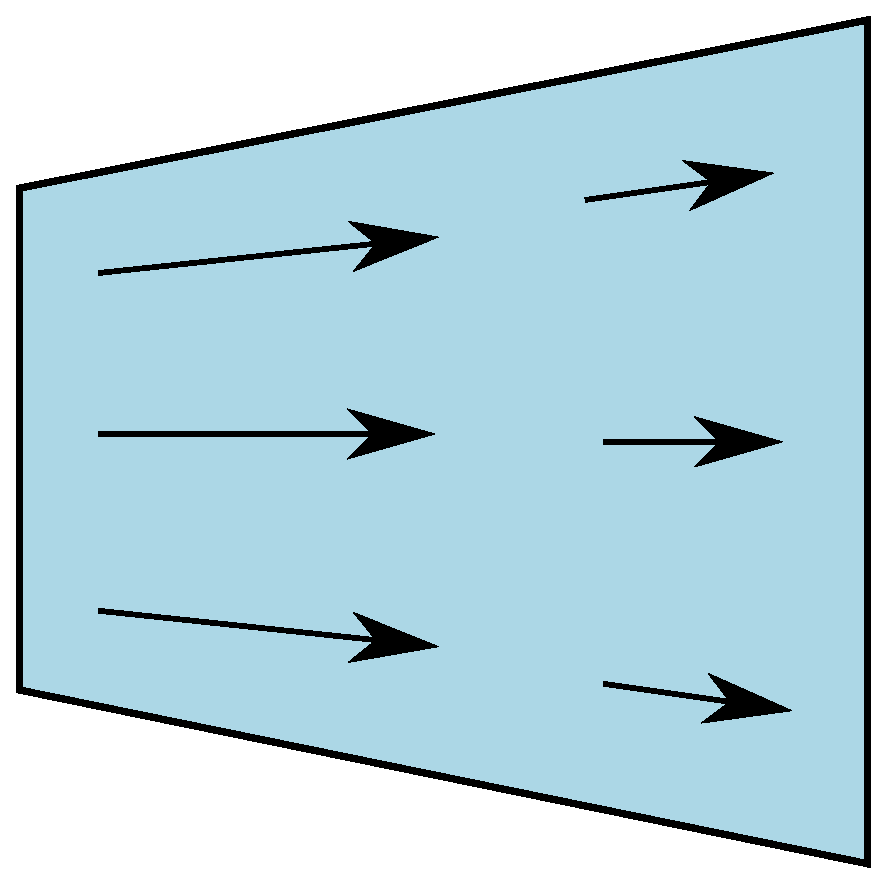
\includegraphics[scale=0.25]{me20b028/me20b028.eps}
\end{center}
\caption{An example of convection}
\label{fig:convection} 
\end{figure}

In Figure~\ref{fig:convection}, though the flow may be steady, the fluid decelerates as it moves down the diverging duct.

%\bibliography{me20b028}
%\bibliographystyle{plain}
